\chapter{Proposed Approach}

Our work builds upon certain aspects of the previous research while introducing a novel and more innovative method for predicting movement origins using machine learning. 
Similar to the previous approach, the pipeline to reach the 20-joints skeleton remains the same (see Sections \ref{sec:orig_markers}, \ref{sec:reduced_markers}).

We chose to utilize a subset of the previous dataset (the one used in \cite{kolykhalova:2020}), and also increase the number of samples by manually annotating videos from other internal resources provided by Casa Paganini \cite{casaPaganini}.\\ 
This choice has been motivated by the necessity to have many short samples that clearly present an origin of movement instead of few samples that are hard to infer in terms of origin of movement, in order to 
reach a high-quality data that can be used in machine learning techniques that will be explained in Section \ref{sec:ml_method}.\\
Another modifica che abbiamo fatto al precedente lavoro è stato confrontare due metodi di misura di similarità, quello implementato nel lavoro originale e la Cosine Similarity (concept explained in Section \ref{subsec:cosine_sim})
Inoltre abbiamo ridotto la teoria dei giochi a semplice weighted degree centrality per velocizzare la pipeline ed evitare il calcolo di $20!$ coalizioni.\\
Infine abbiamo spostato la convalidazione dei frammenti a inizio pipeline utilizzando un meccanismo di validazione a più step tra annotatori esperti e non, di modo da ridurre al minimo l'effetto che i bias avrebbero potuto introdurre nel modello che poi avremmo utilizzato.

TODO DECIDERE SE COENS KAPPA
Furthermore for visualization purposes we implemented a method to prevent inconsistent coloring behaviours among clusters over time, by introducing a novel cluster stabilization algorithm. 

\section{Roadmap}
From the starting point of our work \cite{kolykhalova:2020}, we re-implemented, improved and modified it to compare the method for identifying the origin of movement obtained based on graphs with our new machine learning-based approach.
The roadmap of this thesis can be outlined as follows: \\
The dataset was initially acquired through manual annotation of movement origins in numerous MoCap videos. 
The results were validated by achieving consensus among multiple annotators. 
Additionally, markers for videos lacking previous labeling were manually assigned and subsequently compressed into clusters.
The central objectives of this thesis encompass the development of three main objectives.\\
A \textbf{Cluster Stabilization Algorithm} which ensure that clusters representing groups of related markers or joints, maintain their consistency and coherence over time.
This first one is just for visualization purposes and does not implement a classification method that can be compared with the others.\\
A \textbf{Graph-based Procedure} to recognize the Origin of Movement by identifying key nodes that play pivotal roles in the motion analysis using an algorithmic method that has been handcrafted for this dataset.\\
A \textbf{Machine Learning Model} that perform the same classification task as the previous, but automatically recognizes patterns within the data, without explicitly coding them by hand.

Given the multifaceted objectives, two parallel pipelines were developed.\\
The algorithmic pipeline encompasses several more steps than the other. 
Initially, we smooth the time series of each sample of movement in order to clean the data from impurities such as noise, missing data for markers occlusion or tracking errors that could end up creating unnatural accelerations of some markers. 
Subsequently, we extract physical derived measurements from the trajectories, like the speed, acceleration and angular momentum from the smoothed data. 
Then, employing a model of human body joints, we apply cosine similarity to connected pairs of joints. 
This aids in clustering joints within each movement frame. 
The primary aim at this stage is to ensure the stability of color changes within these clusters. 
Additionally, we construct a secondary graph, where nodes at cluster borders are interconnected and weighted based on their connections across all frames.

The machine learning pipeline follows a different approach on the data. 
We start by normalizing the dataset concerning segment length, the performer's body structure (Skeleton Barycenter and Joints Distance), and the complete movement trajectory. 
Following this, we extract a diverse set of pertinent features from this normalized dataset. These extracted features are then utilized to train a machine learning model, whose performance is thoroughly evaluated using diverse metrics.

Eventually, the outcomes from each pipeline are compared and contrasted to discern their respective effectiveness.

The first pipeline is composed of 
\begin{itemize}
    \item Smoothing the time series of each movement using two classical smoothing algorithms.
    \item Extracting physical measurements from the smoothed data.
    \item Applying cosine similarity to pairs of joints linked by arcs based on a model of physical joints in the human body.
    \item Clustering joints for each frame of the movement.
    \item The primary objective here was the temporal stabilization of cluster color changes.
    \item Formation of a second graph with nodes at cluster borders, connected to other clusters. These nodes are weighted based on their connections and ranked across all frames.
\end{itemize}
The second pipeline involved:
\begin{itemize}
    \item Normalizing the dataset in terms of segment length (Time series Sampling), performer's body structure (Skeleton Barycenter and Joints Distance), and the entire trajectory of the movement.
    \item Extracting a wide range of relevant features from the normalized dataset.
    \item Using these features to train a machine learning model.
    \item Evaluating the model's performance using various metrics.
\end{itemize}
Finally, the results from each pipeline are compared.

\clearpage
\begin{figure}[H]
    \centering
    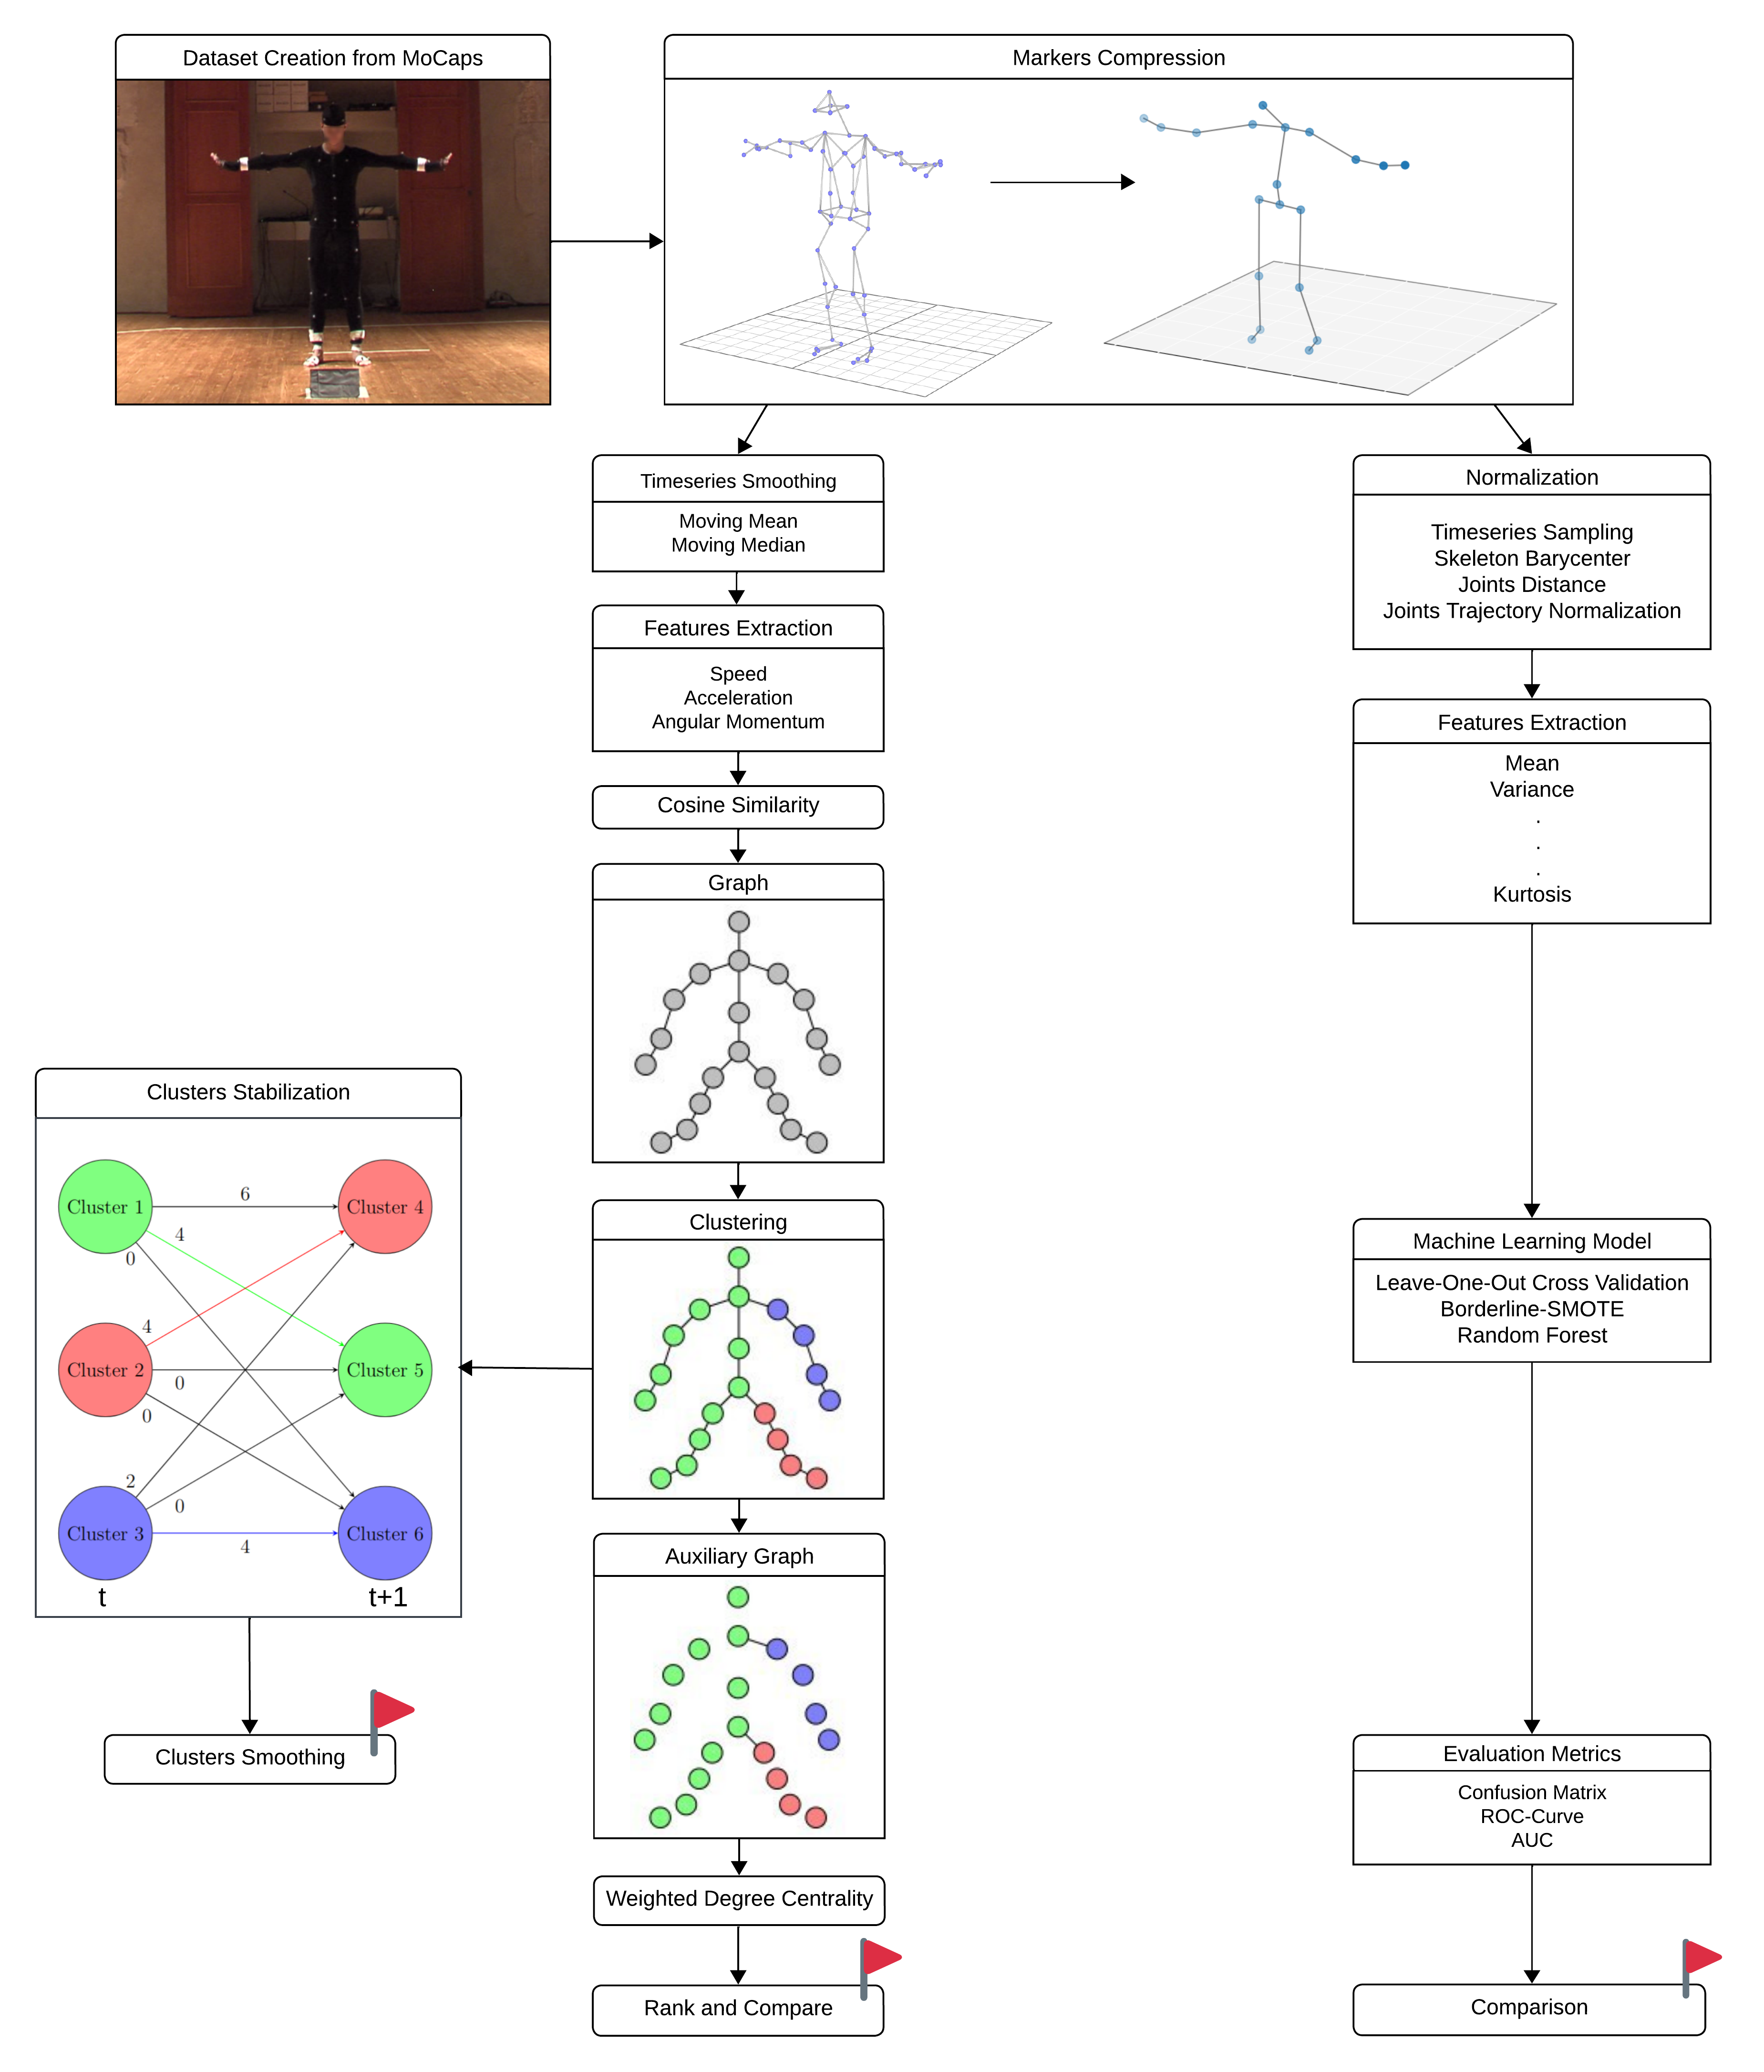
\includegraphics[width=\textwidth,height=\textheight,keepaspectratio]{Walkthrough.png}
    \caption{Roadmap of this Thesis}
    \label{fig:walktrough}
\end{figure}